I will now discuss the results of my implementation of the algorithm and the implemented Hamiltonians.
The code is written in Python 3.8, while for the semidefinite program the interface PICOS is used.
All the code can be found in appendix A.
To produce informative plots, the implementation executes the algorithm with output $y$ (Bloch vector) and computes the ratio $r=y^{T}Cy/\lambda_{max}$.
It does this $o$ times per number of qubits $n$.
The average of the $o$ ratios per $n$ is plotted, where a logarithmic scale is used for the $x$-axis.
The variance has been visualized as error bars.
I have chosen to plot in the range of $n=4$ to $n=5200$ in $25$ equidistant steps on the logarithmic scale, using $o=20$.
The computation time became infeasible for larger qubit numbers, as the complexity of the function \emph{numpy.linalg.eig()}, used to to find the solution vectors, is $O\left(N^3\right) $.
Secondly, I have done the same computation but instead of taking the average of the lists, I have picked the maximal approximation ratio and plotted it.
While this does not specifically test the code for the behaviour of the approximation ratio, it provides information on the practical uses of the algorithm.
The solutions to the SDP were implemented in numpy, using the fact that the objective function $Tr(CM)=\sum_{i,j}C_{ij}M_{ij}$ admits the periodic patterns of the Hamiltonians.
For the plots shown in this thesis I have used $c=2$.
The next steps of implementation would include finding the solution vectors by hand, reducing the complexity of the algorithm dramatically, and analyzing the constant $c$.
This however was not possible in the timeframe of this thesis.\\
The Ising model with a transverse field has physical relevance because it can be used to study quantum phase transitions of ferroelectrics with a tunneling effect or systems of interacting magnetic spins with an outer field.
The Hamiltonian
\[
H=\alpha \sum_{i} Z_i + \beta \sum_{i} X_iX_{i+1}
\]
has been exactly solved in one dimension \cite{pfeuty70}.
One way to do this by transforming the Hamiltonian into a quadratic form of Fermi operators via the Jordan-Wigner transformation \cite{nielsen05}.
To diagonalize this Hamiltonian, one can use the Bogoliubov transformation which is an isomorphism in the canonical commutation or anticommutation relation algebra \cite{bogoljubov58}.\\
The parameter $\alpha$ corresponds to the tunneling energy and $\beta$ to the nearest neighbour interaction in the ferroelectric problem.
We here look at a closed chain, meaning $1\le i \le n, \quad X_{n+1}=X_{1}$.
I have first implemented the model with $\alpha =0, \quad \beta =1$.
This is a model of a one-dimensional chain with nearest neighbour interaction without an outer field.
The state that is stabilized by all terms simultaneously is the state achieving the maximal eigenvalue.
In this case, it is the $n$-fold tensor product of the $+1$-eigenvector of $X$: \[
	\ket{\psi}= \ket{+}_1\otimes\ket{+}\otimes\ldots\otimes\ket{+}_n
,\] where \[
\ket{+}_i= \frac{\ket{0}_i+\ket{1}_i}{\sqrt{2}}
.\]
The maximal eigenvalue of the Hamiltonian is therefore $\lambda_{max}=n$, since it has $n$ terms.
Figure \ref{fig:1} shows the result of computing numeric values of the approximation ratio over a range of $n$ qubit Hamiltonians of this kind.
\begin{figure}[H]
	\centering
	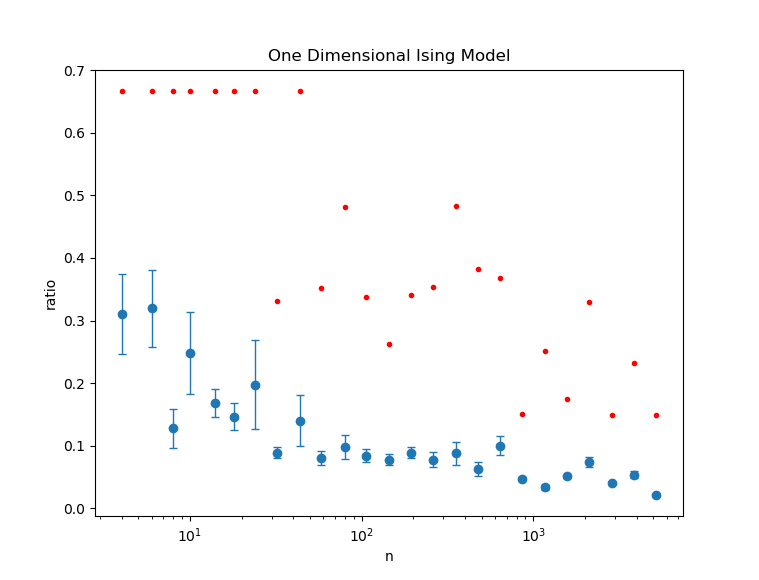
\includegraphics[width=0.9\textwidth]{avgchainplot(4,5200,2,20,25)}
	\caption{The average of $20$ approximation ratios per $n$, plotted from $4$ to $5200$ qubits with logarithmic scale on the $x$-axis for the one dimensional Ising model with no transverse field. The red points represent the maxima of the respective iterations.}
	\label{fig:1}
\end{figure}
\noindent While we can only be sure for significantly larger qubit numbers, it seems to exhibit the expected behaviour of $\Omega(\frac{1}{\log{}n})$.\\
I have also implemented the transverse field Ising model for non-zero $\alpha$ and arbitrary $\beta$.
To compute the maximal eigenvalue, I have followed \cite{pfeuty70}.
Since the Hamiltonian has terms that are linear in Pauli operators, we have to transform it as discussed in chapter 4.
The Hamiltonian that was implemented is \[
H = H_2 + Z_{n+1}H_1 =\alpha Z_{n+1}\sum_{i} Z_i + \beta \sum_{i} X_iX_{i+1}
.\]
Fig. \ref{fig:2} shows a result of implementing this model for several ratios $\lambda= \frac{\alpha}{\beta}$.
\begin{figure}[H]
	\centering
	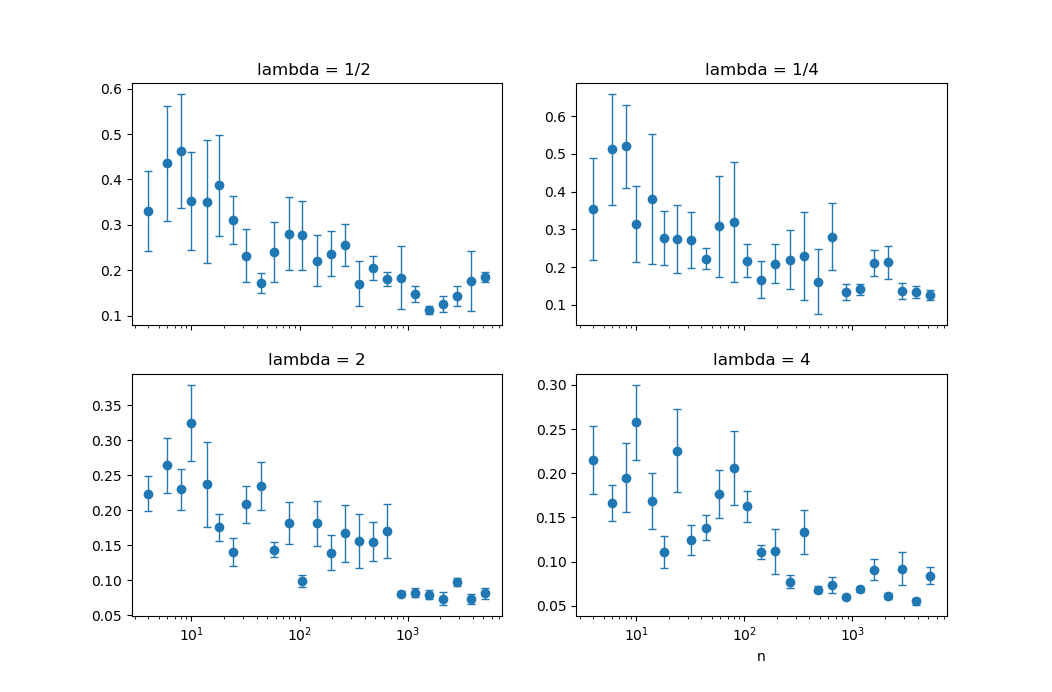
\includegraphics[width=1.1\textwidth]{tfiplots}
	\caption{The average of $20$ approximation ratios per $n$, plotted from $4$ to $5200$ qubits with logarithmic scale on the $x$-axis for the transverse field Ising model for several ratios $\lambda$}
	\label{fig:2}
\end{figure}

\noindent While the behaviour is more scattered in this case, the plot shows a similar behaviour to figure \ref{fig:1}.
The variance is larger, but diminishes for larger $n$.
To be able to accurately see the predicted behaviour, we would have to compute significantly larger $n$.\\\newpage
\noindent The second model implemented is \[
	H =  X_1X_{2}+Z_1Z_{2}+X_{3}+X_{4}+X_5X_{6}+Z_5Z_{6}+X_{7}+X_{8}\ldots
,\]
where we restrict $n$ to be a multiple of $4$.
In contrast to the Ising model without a transverse field, the maximal eigenvalue can not be achieved by a product state in this case.
To find out the maximal eigenvalue lets look at the first two quadratic terms:
\[
H_2=X_1X_2+Z_1Z_2
.\]
The state achieving the maximal eigenvalue $\lambda_{max}(H_2)=2$ is the EPR-state $\ket{\text{EPR}}=\frac{\bra{00}+\bra{11}}{\sqrt{2}}$.
This is a maximally entangled state.
To find out the product state which approximates this best, maximize the overlap with a general product state:
\[
	\ket{\psi}=\ket{\psi_1}\otimes\ket{\psi_2}=\left(a_1\ket{0}+b_1\ket{1}\right)\otimes\left(a_2\ket{0}+b_2\ket{1}\right)
\] with $a_1^2+b_1^2=a_2+b_2^2=1$.
The overlap is then:\[
\max_{\psi_1,\psi_2}\left(\left|\braket{\text{EPR}}{\psi}\right|^2\right)=\max\left(\left|\frac{1}{\sqrt{2}}\left(a_1a_2+b_1b_2\right)\right|^2\right)=\frac{1}{2}
,\]
with either $a_1=a_2=1$ and $b_1=b_2=0$ or $b_1=b_2=1$ and $a_1=a_2=0$.
Therefore, the product states with the maximal overlap are $\ket{00}$ and $\ket{11}$ with maximal eigenvalue $\lambda_{sep}(H_2)=1$, the approximation ratio being  $\frac{\lambda_{sep}H(2)}{\lambda_{max}(H_2)} = 0.5$.\\
In general the maximal eigenvalue of the Hamiltonian is therefore $\lambda_{max}(H)=n$, and the best achievable eigenvalue by a product state is $\lambda_{sep}(H)=\frac{3}{4}n$.
Fig. \ref{fig:3} seems to show the expected $\Omega\left( \frac{1}{\log{}n} \right) $ approximation ratio:
\begin{figure}[h]
	\centering
	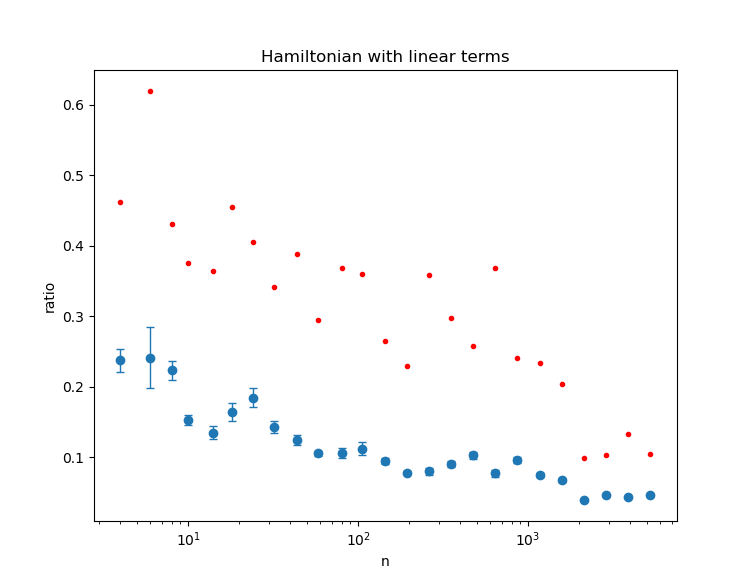
\includegraphics[width=0.9\textwidth]{avgplot(4,5200,2,20,25}
	\caption{The average of $20$ approximation ratios per $n$, plotted from $4$ to $5200$ qubits with logarithmic scale on the $x$-axis for a chain with linear terms. The red points represent the maxima of the respective iterations.}
	\label{fig:3}
\end{figure}
\noindent Since the functionality and efficiency of this algorithm has been proved, the purpose of the implementation of the two models were of course mainly for testing the code itself.
